\section{Оборудование и инструментальные погрешности}

Мосент иннерции можно определить при помощи установки, изображённой на рисунке
(трифилярного подвеса). Оно состоит из неподвижной платформы $P$, к которой на трёх
симметричных нитях подвешена вращающаяся платформа $P'$. Верхнюю платформу можно
повернуть при помощи рычага, после чего возникают колебания.

\begin{figure}[ht!]
    \centering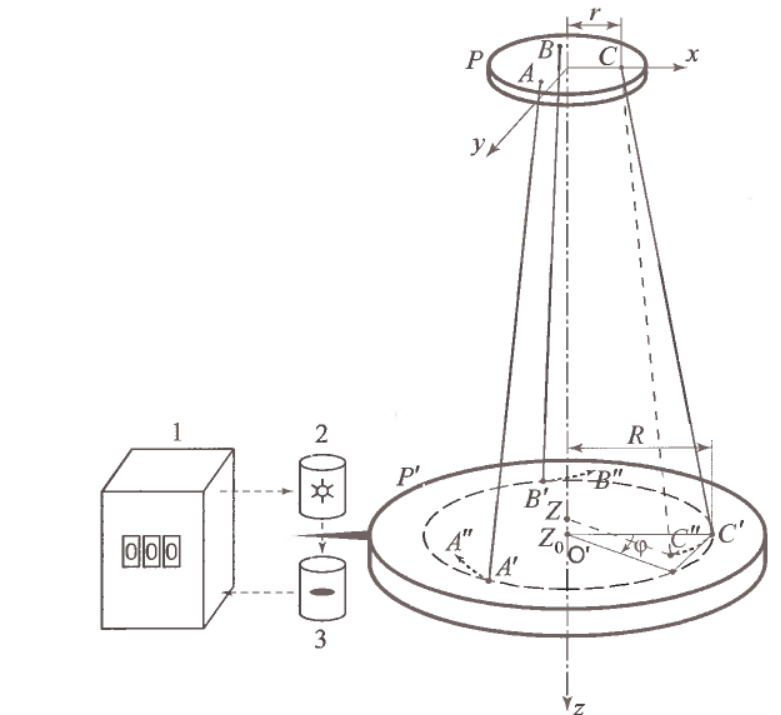
\includegraphics[width=0.8\linewidth]{img/podves.png}
\end{figure}

Если пренебречь потерями энергии, то закон сохранения энергии можно записать как
\[\frac{I\dot{\varphi}^2}{2}+mg\left(z_0-z\right)=E\]
$I$~--- момент иннерции платформы вместе с телом, $\varphi$~--- угол поворота платформы
от положения равновесия, $z_0$~--- координата по вертикали центра нижней платформы в
равновесии, $z$~--- координата этой точки, $E$~--- полная механическая энергия системы.

Выразим $z$ через угол поворота
\[z\approx z_0-\frac{Rr\varphi^2}{2z_0}\]

Тогда закон сохранения энергии
\[\frac{1}{2}I\dot{\varphi}^2+mg\frac{Rr}{2z_0}\varphi^2=E\]
\[I\ddot{\varphi}+mg\frac{Rr}{z_0}\varphi=0\]
Это уравнение гармонических колебаний с периодом
\[T=2\pi\sqrt{\frac{Iz_0}{mgRr}}\]
\[I=\frac{mgRrT^2}{4\pi^2z_0}\]
\[I=kmT^2\]
где $k=\frac{gRr}{4\pi^2z_0}$~--- постоянная величина для данной установки.

Затухание колебаний должно быть мало (время затухания в 2 раза много больше периода).
Период колебаний рекомендуется определять с относительной погрешностью $0{,}5\%$.

Для подсчёта числа колебаний используется счётчик.
